\documentclass[11pt]{article}
\usepackage[margin=1.1in]{geometry}
\usepackage{amsmath,amssymb,amsthm}
\usepackage{graphicx}
\usepackage{booktabs}
\usepackage[hidelinks]{hyperref}

\newtheorem{proposition}{Proposition}
\theoremstyle{remark}
\newtheorem{remark}{Remark}

\newcommand{\E}{\mathbb{E}}
\newcommand{\Prob}{\mathbb{P}}

\title{Deterministic Choice Probabilities and Share Inversion\\
for Factor Probit with Many Alternatives}
\author{Peter Cotton\thanks{Numbers in this paper are produced by committed, seeded
scripts with correctness anchors run before any comparison
(\url{https://github.com/microprediction/kinetics}, experiments 13--16; an
immutable commit will be pinned at submission). The algorithm ships in the
\texttt{thurstone} package; package--benchmark agreement is itself a reported
number. Benchmarks: Apple M4, 16\,GB, Python 3.12.9, NumPy 2.4.6, SciPy
1.18.0, single-threaded; timings are single realizations without warm-up
medians; peak memory below 2\,GB.}}
\date{August 2026 --- working draft, revised}

\begin{document}
\maketitle

\begin{abstract}
Multinomial probit choice probabilities are high-dimensional Gaussian integrals
with no closed form; the standard tool, the GHK simulator, computes them one
alternative at a time by smoothed importance sampling. For the factor-structured
case $\Sigma = VV^\top + \mathrm{diag}(D)$ we describe a deterministic method
that computes \emph{all} $N$ probabilities together: conditionally on $k$
Gaussian factors the alternatives are independent, and a lattice
survival-product identity yields the entire share vector in $O(QNL)$ for $Q$
quadrature nodes and $L$ lattice points --- deterministic quadrature at low
factor rank, reproducible fixed-seed RQMC at higher rank. In the tested $k=2$
problems the method had observed maximum discrepancy below $10^{-3}$ from the
stated simulation references, from $N=5$ to $N=5000$ (22 seconds at $N=5000$,
where the reference's own noise is of comparable order), and became faster
than our reference GHK implementation near $N=200$; extrapolating that
implementation's timing and $R^{-1/2}$ accuracy suggests hours, not seconds,
at matched error for $N=5000$. A direct utility simulator at matched wall
time reaches errors within a factor of $1.3$--$3$ at these budgets, so at the
$10^{-3}$ level the case for the method is not raw forward speed but error
decay, reproducibility, resampling-free derivatives, and inversion. Because
the approximation is reproducible and differentiable without resampling, it supports
practical market-share inversion (a Jacobi-style diagonal-Newton fixed point;
$N=1000$ in under a minute) and reuse of the conditional field for all $N$
single-removal counterfactuals in $O(QN^2L)$. Boundary experiments are reported
as they fell: on dense covariances with three spectral-decay profiles, the
rank-8 approximation matched or beat GHK at $R=10^4$ throughout the tested
size, and in a substitution study with all noise families standardized to unit
variance, factor structure supplied the larger accuracy increment on
high-mass deletions while family and factor increments were comparable on
mid-mass deletions, in this Gaussian-adjacent design.
\end{abstract}

\section{Introduction}

The multinomial probit (MNP) model computes choice among $N$ alternatives with
jointly normal utilities, allowing flexible substitution patterns --- the
property that plain multinomial logit trades away for tractability. Its
probabilities are $(N-1)$-dimensional Gaussian orthant integrals. The field's
workhorse for three decades has been the GHK simulator
\cite{geweke1994,hajivassiliou1998,train2009}: smoothed importance sampling
along a Cholesky factor, one alternative at a time. GHK is accurate and well
understood at moderate $N$; its structural costs are that error decays as
$R^{-1/2}$ in the number of draws, that the full share vector requires a
separate computation per alternative, and that each evaluation is a
finite-simulation approximation whose characteristics enter derivative-based
estimation (Section~\ref{sec:benchmark}).

This paper concerns the factor-structured case
\begin{equation}
U_i \;=\; \mu_i + v_i^\top f + \sqrt{D_i}\,\varepsilon_i,
\qquad f \sim N(0, I_k), \quad \varepsilon_i \sim N(0,1) \text{ i.i.d.},
\quad D_i > 0,
\label{eq:model}
\end{equation}
i.e.\ $\Sigma = VV^\top + \mathrm{diag}(D)$ --- the form in which applied
covariance structure often arrives. Factor dimension reduction for probit is
itself classical: one-factor quadrature goes back to Butler and Moffitt
\cite{butler1982}, and factor-analytic probit to Elrod and Keane
\cite{elrod1995}. What appears not to have been assembled is the
\emph{all-alternatives} computation: conditionally on the factors, a lattice
survival-product identity \cite{cotton2021} computes every alternative's
one-dimensional integral in a single $O(NL)$ pass --- the field survival
product is built once and each alternative's leave-one-out field is recovered
by division. A $k$-dimensional quadrature around that inner loop gives the
whole share vector deterministically. The contribution here is that assembly,
its inverse (share-to-utility) transform, the reuse of the conditional field
for removal counterfactuals, and benchmark plus boundary evidence.

\begin{proposition}[Conditional identity]\label{prop:identity}
Under \eqref{eq:model}, with $g_i(\cdot \mid f)$ and $F_i(\cdot \mid f)$
the conditional density and CDF of $U_i$ given $f$,
\begin{equation}
p_i \;=\; \E_f\!\left[\;\int g_i(x \mid f)
\prod_{j \neq i} F_j(x \mid f)\, dx \right],
\qquad \sum_i p_i = 1,
\label{eq:forward}
\end{equation}
and the product over $j \ne i$, for all $i$ simultaneously, is obtained from
$\log F_{\mathrm{field}} = \sum_j \log F_j$ by subtraction.
\end{proposition}
\begin{proof}
Conditional on $f$ the $U_j$ are independent, so $\Prob(U_i \text{ maximal}
\mid f) = \int g_i \prod_{j\ne i} F_j\,dx$; average over $f$. The events
partition (ties are null for continuous laws), giving $\sum_i p_i = 1$.
\end{proof}

\begin{proposition}[Complexity]\label{prop:complexity}
With $Q$ factor nodes and $L$ lattice points, the forward share vector costs
$O(QNL)$; the full single-removal ensemble $\{P(j \text{ chosen} \mid i
\text{ removed})\}_{i,j}$ costs $O(QN^2L)$ arithmetic and $O(N^2)$ storage,
reusing one conditional field construction.
\end{proposition}
\begin{proof}
Per node: the field log-product costs $O(NL)$, each alternative's integral
$O(L)$ after subtraction, giving $O(NL)$; the removal ensemble evaluates $N$
survivor integrals for each of $N$ removals, $O(N^2L)$, over the same cached
field.
\end{proof}

\begin{proposition}[Identification and differentiability]\label{prop:ident}
$p(\mu + c\mathbf{1}) = p(\mu)$, so $J = \partial p/\partial \mu$ has
$\mathbf{1}$ in its null space and $\mu$ is identified only up to location.
With $B$ an $N \times (N-1)$ basis of $\mathbf{1}^\perp$ and $\mu = B\eta$,
share inversion and implicit differentiation are taken in reduced coordinates:
$d\eta/d\theta = -(B^\top J B)^{-1} B^\top \partial p/\partial\theta$,
provided $B^\top J B$ is nonsingular.
\end{proposition}
\begin{proof}
Invariance holds because a common location shift does not change the argmax;
differentiating $p(\mu + c\mathbf{1}) = p(\mu)$ in $c$ gives $J\mathbf{1} =
0$. Differentiating $p(B\eta(\theta), \theta) = \hat p$ in $\theta$ and
projecting with $B^\top$ gives the reduced formula under the stated
regularity.
\end{proof}
\begin{remark}
For the Gaussian model with $D_i > 0$, $p(\mu) = \nabla_\mu G(\mu)$ for the
social-surplus function $G(\mu) = \E \max_i \{\mu_i + \xi_i\}$; strict
convexity of $G$ on $\mathbf{1}^\perp$ would give injectivity of the share
map modulo location and, with a coercivity argument, existence and uniqueness
of the inverse for every strictly positive target. We use this only as
motivation here; a proof is future work.
\end{remark}

\begin{proposition}[Jacobian--vector products in $O(QNL)$]\label{prop:jvp}
For a direction $h$, let $A(x, f) = \sum_j h_j\, \partial_{a_j} \log
S_j(x \mid f)$ in the reflected (min-wins) coordinates $a$. Then
\[
(Jh)_i \;=\; \E_f \int R_i \left[\, h_i\, \partial_{a_i} g_i
+ g_i \left( A - h_i\, \partial_{a_i} \log S_i \right) \right] dx,
\qquad R_i = \prod_{j \ne i} S_j,
\]
where the field sum $A$ is formed once per node and lattice location, so all
$N$ components cost $O(NL)$ per node. (Verified against central finite
differences to $8\times10^{-9}$; implemented and tested in the repository.)
This enables Krylov solves of the reduced system in
Proposition~\ref{prop:ident} without forming $J$ densely at $O(QN^2L)$.
\end{proposition}

The factors need not be Gaussian: \eqref{eq:forward} requires only
conditional independence and an integrable factor law, so Student, mixture,
or empirical factor distributions are admissible with appropriate nodes, and
the base densities may be arbitrary and alternative-specific. One caution for
asymmetric laws: the implementation works in the reflected (min-wins)
race, and $-U$ has the same distribution as the reflected model only when the
factor and base laws are symmetric; for asymmetric laws the reflected
distributions must be used explicitly.

\paragraph{Numerical method, stated completely.} The benchmarks use $L = 1501$
lattice points on the adaptive interval
$[\min_{i,q} m_i(f_q) - 8\max_i\sqrt{D_i},\,
\max_{i,q} m_i(f_q) + 8\max_i\sqrt{D_i}]$, where $q = 1, \dots, Q$ indexes
the retained factor nodes. Factor integration: the GHK benchmark (experiment
13) uses product Gauss--Hermite of order 15/11/9 for $k = 2/3/4$; the boundary
experiment (experiment 14) uses order 15 per dimension for all $k \le 4$,
which after pruning weights below $10^{-7}$ of the maximum leaves $Q = 145$,
$1317$, and $10929$ nodes for $k = 2, 3, 4$ --- making the exponential growth
of $Q$ with rank explicit; scrambled-Sobol nodes ($2^{13}$ points, fixed seed)
are used for $k > 4$: reproducible fixed-seed randomized QMC, disclosed as
such. Survival floors sit at $10^{-300}$ and the quadrature output is
normalized by its sum. The returned map is a reproducible, piecewise-smooth
numerical approximation of \eqref{eq:forward}; statements about derivatives
refer to derivatives of this approximation, whose fidelity to exact MNP
derivatives is governed by $L$ and $Q$.

\paragraph{Inversion.} Given target shares $\hat p$ and $(V, D)$, the inverse
transform finds mean-zero $\mu$ with $p(\mu) = \hat p$ by a damped Jacobi-style
diagonal-Newton iteration: all coordinates updated simultaneously using
own-location slopes of the unnormalized lattice map (available from the same
pass), the field refrozen each iteration, a warm start from the
independent-field inverse using total variances, and a tail-aware tolerance
(alternatives with target shares below $10^{-4}/N$ are matched best-effort;
their locations are weakly identified --- itself a conditioning caution for
the reduced Jacobian when shares are tiny or alternatives nearly collinear).
Convergence in a handful of iterations is an empirical observation on the
tested problems, not a theorem. The design follows the original transform's
inversion \cite{cotton2021} and the calibration practice of
\cite{allocationpkg}.

\section{Benchmark against GHK}\label{sec:benchmark}

Anchors first. On the binary case, where MNP has a closed form, the lattice
transform agrees to $3\times10^{-16}$ and our GHK implementation --- validated
before being compared against --- to $2\times10^{-14}$ at $R = 2\times10^5$
(an easy anchor for both methods, useful for code validation rather than as
evidence about the hard regime). At $N=5$ both methods sit within the noise of
a $10^7$-draw Monte Carlo reference, and the shipped
\texttt{thurstone.FactorRace} agrees with the benchmark kernel to
$1.1\times10^{-5}$.

Error metric: throughout, $\max_i |\hat p_i - p_i|$ against a simulation
reference. A maximum over $N$ coordinates tends to grow with $N$ at fixed
per-coordinate accuracy, and the reference's own maximum-coordinate noise
behaves likewise; mean-absolute and total-variation summaries are committed
alongside (experiment 16): at $N=1000$ the lattice's mean absolute error is
$6\times10^{-6}$ and total variation $3.1\times10^{-3}$ against a fresh
$2\times10^6$-draw reference.

\begin{table}[h]
\centering
\begin{tabular}{lcc}
\toprule
$N$ & lattice transform & GHK ($R=1000$) \\
\midrule
5 & 21 ms, err $4.1\times10^{-4}$ & 1 ms, err $3.1\times10^{-3}$ \\
20 & 95 ms, err $3.8\times10^{-4}$ & 12 ms, err $4.4\times10^{-3}$ \\
50 & 257 ms, err $2.1\times10^{-4}$ & 77 ms, err $7.7\times10^{-3}$ \\
200 & 930 ms, err $2.8\times10^{-4}$ & 1333 ms, err $6.7\times10^{-3}$ \\
1000 & 4.5 s, err $8.0\times10^{-4}$\,$\dagger$ & --- \\
5000 & 22.6 s, err $9.0\times10^{-4}$\,$\dagger$ & --- \\
\bottomrule
\end{tabular}
\caption{Full share vector, $k=2$ factors, one problem per size (utility
spread 1.0 through $N=200$, 1.5 above). Reference: $2\times10^6$ MC draws
through $N=200$; $5\times10^5$ draws at $N=1000$ and $5000$ ($\dagger$: there
the reference's own maximum-coordinate noise is of comparable order, so these
entries bound the lattice error only to that order). A replication study at
common spread 1.0 (experiment 16; ten problems per size at $N \le 200$, three
at $N=1000$, twin independent $2\times10^6$-draw references per problem)
gives worst-case lattice error $2.9$--$3.6\times10^{-4}$ at every size, at or
below the references' own replicate-to-replicate noise. Lattice error stayed
below $10^{-3}$ throughout; GHK cost crossed over by $N \approx 200$.}
\label{tab:frontier}
\end{table}

\paragraph{Matched-accuracy extrapolation (not a measurement).} Fitting a
power law to the reference implementation's timings over $N \in [20, 200]$
($\alpha \approx 2.0$; a lower bound, the asymptotic per-share cost being
cubic) and combining with $R^{-1/2}$ error scaling suggests that matching the
lattice's $9\times10^{-4}$ at $N=5000$ would take this implementation on the
order of twelve hours, against 22 seconds. The baseline is a straightforward
single-threaded Python GHK: per-alternative Cholesky, plain pseudorandom
uniforms, one realization per problem, shares normalized by their sum. It
establishes the scaling of the per-alternative simulation approach, not a
field-wide impossibility. The strongest cheap baseline is \emph{direct
utility simulation} --- draw utilities, take argmax, average --- which
produces the whole share vector per draw and, unlike GHK, does not pay per
alternative. We ran it at wall time matched to the lattice call (experiment
16): its maximum-coordinate error was within a factor of $1.3$--$3$ of the
lattice's at every tested $N$ ($7.2\times10^{-4}$ versus $4.9\times10^{-4}$
at $N=1000$, $0.6$M draws in the matched 4.4 seconds). At the $10^{-3}$
accuracy level, then, raw forward speed does not by itself separate the
methods; what does is error decay ($R^{-1/2}$ against spectral-in-$L$,
so each added decimal digit costs $100\times$ in draws against a linear
lattice refinement), reproducibility, resampling-free derivatives, and the
inversion and removal machinery below. Remaining stronger baselines ---
QMC-GHK, seed-replicated uncertainty bands, minimax tilting \cite{botev2017}
--- are queued in the repository.

\begin{figure}[h]
\centering
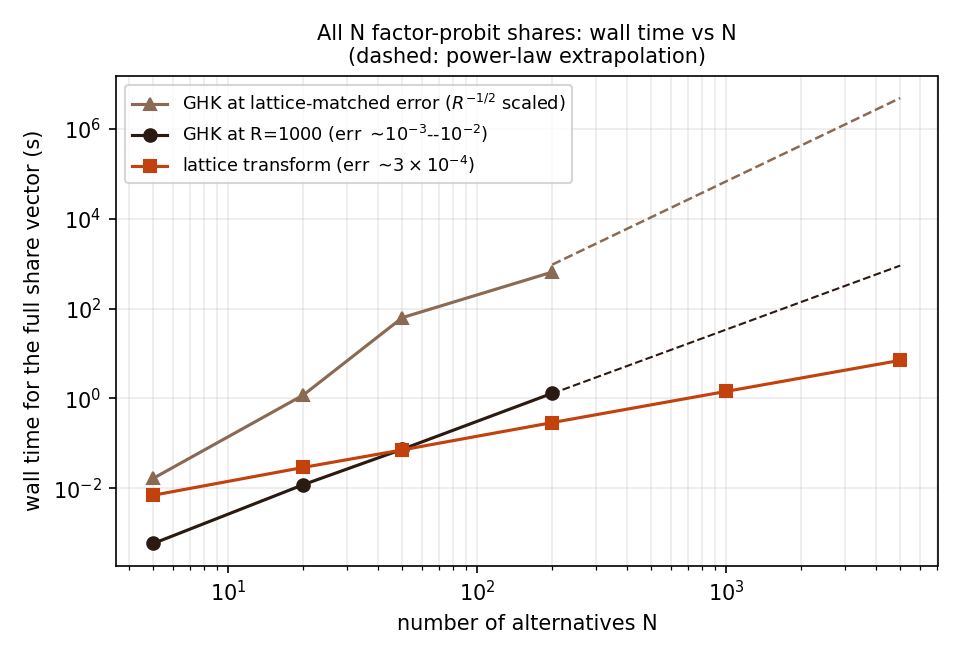
\includegraphics[width=0.48\textwidth]{figs/frontier.png}\hfill
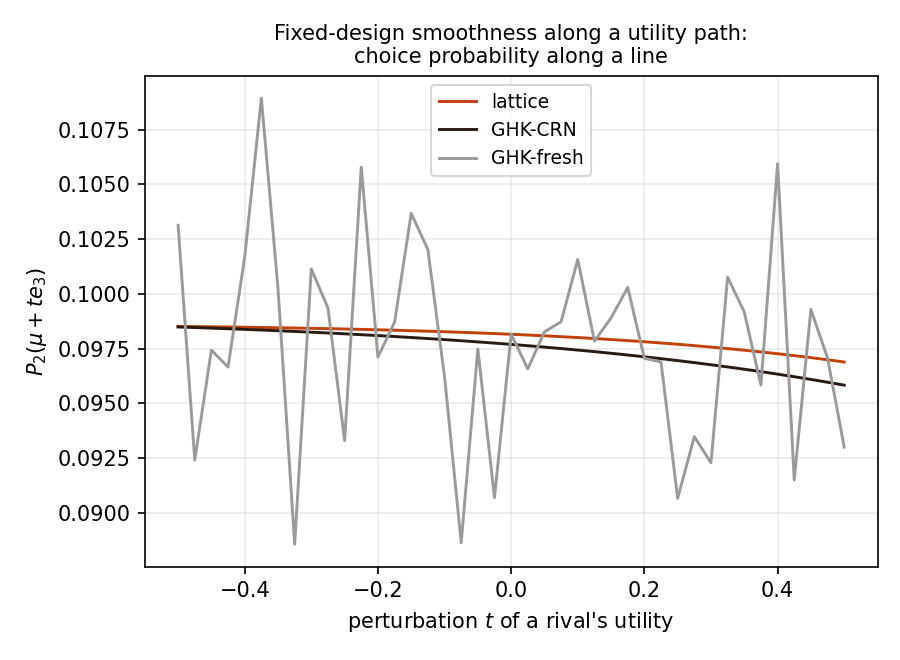
\includegraphics[width=0.48\textwidth]{figs/smoothness.png}
\caption{Left: wall time for the full share vector (log--log). Right: a choice
probability along a line in utility space. Fresh-draw GHK shows run-to-run
simulation noise (roughness statistic --- maximum second difference over
$dt^2$ --- 39.3 vs.\ 0.01); common-random-number GHK is a smooth
deterministic approximation conditional on its draw set, and its curve
differs visibly from the lattice curve --- a discrepancy between two
approximations whose decomposition requires an independent high-accuracy
reference, queued. All three are approximations.}
\label{fig:frontier}
\end{figure}

\paragraph{Derivatives, stated correctly.} For fixed factor nodes and a fixed
lattice, the transform is a reproducible, (piecewise-)differentiable function
of $\mu$ whose derivatives are evaluated without resampling; analytic
own-location slopes of the unnormalized map come from the same pass and serve
as the inversion preconditioner. These are derivatives of the numerical
approximation, not exact MNP derivatives, and GHK-based practice likewise
differentiates its approximation, analytically or with fixed draws
\cite{hajivassiliou1998,train2009}. The practical distinction is the character
and controllability of the approximation error --- quadrature resolution
versus draw count --- not the possibility of differentiation.

\paragraph{Share inversion.} At $N=1000$, $k=2$, with targets from
$5\times10^6$ MC draws floored at $10^{-7}$ and renormalized: the inversion
completes in 59 seconds. The iteration solves its own equations to
$6.3\times10^{-9}$ --- a statement about the solver, not statistical accuracy,
since the target carries sampling noise $\sim\!2\times10^{-4}$ --- and
recovers the utilities of identified alternatives (target share above
$3\times10^{-4}$) to maximum error $0.014$. A replication study (experiment
16) repeats the inversion on a second $N=1000$ problem against three
independent $5\times10^6$-draw targets: 58--61 seconds each, the same 162
alternatives identified each time (98.1\% of share mass), recovery error
maximum $0.018$--$0.025$ and median $0.0026$ across replicates, with the
recovery-versus-share curve committed alongside. We are not aware of probit
share inversion at this scale in current simulation-based practice.

\paragraph{Removal ensemble.} All 200 single-removal share vectors from one
conditional field construction in $O(QN^2L)$: 3.7$\times$ faster than an
extrapolation from direct recomputations, with ten evenly spaced removals
checked directly (maximum discrepancy $5.6\times10^{-17}$).

\section{Boundary experiments}\label{sec:boundary}

\paragraph{General covariance through the factor approximation.} The method
requires $\Sigma \approx VV^\top + D$; GHK does not. We generated one random
correlation matrix at each spectral decay $\lambda_m \propto m^{-\gamma}$,
$\gamma \in \{0.5, 1.5, 3\}$, at $N=50$ (single realizations; replication over
matrices and utility vectors is queued), fit factors by iterated principal
factor analysis, and measured share error against an $8\times10^6$-draw
reference, with GHK at the exact $\Sigma$ for comparison. The plotted quantity
is the \emph{rank-$k$ approximation error of the stated fitting and
integration procedure} --- covariance-fit error plus factor-integration and
lattice error --- not a minimum over factor models. Findings as they fell:
error decays fastest for near-low-rank truth ($\gamma=3$: $5.6\times10^{-2}$
at $k=1$ to $1.2\times10^{-3}$ at $k=8$) and slowest at intermediate decay
($\gamma=1.5$: $2.4\times10^{-2}$ to $2.6\times10^{-3}$); at every tested
decay the $k=8$ result (fixed-seed RQMC nodes) matched or beat GHK at
$R=10^4$ ($3.2$--$4.1\times10^{-3}$). We expected a clear GHK-wins regime at
this size and did not find one; where accuracy demands exceed the achievable
rank-$k$ error --- intermediate spectra with $k$ capped, or short-range
correlation at large $N$ --- GHK's arbitrary-$\Sigma$ generality is the right
tool. Further practical boundaries (small $D_{\min}/D_{\max}$, wide utility
ranges, near-perfect correlation, extreme shares) stress the uniform lattice
and are queued as resolution sweeps in $L$ and $Q$.

\paragraph{Substitution fidelity, with noise families standardized.} Why want
probit-style flexibility at scale? Ground truth misspecified for every
candidate: $t(5)$-distributed factors and skew-normal idiosyncratic noise,
\emph{all noise families standardized to mean zero and unit variance}. (An
earlier version of this experiment confounded noise family with noise
variance; the standardized rerun is reported here, and the ordering
survived.) Candidates --- plain logit, factor mixed logit (unit-variance
Gumbel base), factor probit --- are calibrated to identical full-menu shares
with the true loadings supplied (calibration residuals $4.9\times10^{-11}$
and $1.1\times10^{-9}$ on menu shares), and scored on deletion
counterfactuals against fresh simulation truths. Blocks whose removed share
sits at the Monte Carlo noise floor are uninformative (all models tie). Of
24 deletion blocks, one falls in the high-mass stratum and four in the
mid-mass stratum --- small strata, so the numbers below are indicative, not
estimates with useful standard errors. The misallocated fraction of
redistributed mass is:

\begin{center}
\begin{tabular}{lcc}
\toprule
 & deleted mass $>10\%$ & deleted mass 2--10\% \\
\midrule
plain logit (IIA) & 15.9\% & 25.7\% \\
factor mixed logit & 7.7\% & 17.1\% \\
factor probit & \textbf{2.8\%} & \textbf{7.8\%} \\
\bottomrule
\end{tabular}
\end{center}

The precise reading: in the high-mass stratum (a single block), factor
structure supplies the larger increment ($15.9 \to 7.7$, i.e.\ $8.2$ points,
versus $7.7 \to 2.8$, $4.9$ points for the idiosyncratic family); in the
mid-mass stratum (four blocks) the two increments are comparable, with the
family increment slightly larger ($8.6$ versus $9.3$ points). Caveats: the
truth's skew-normal noise is Gaussian-adjacent (favoring probit), and this is
a single design and seed with small strata --- replication across skewness
and tail designs is queued before any general claim.

\begin{figure}[h]
\centering

\includegraphics[width=0.48\textwidth]{figs/full_sigma.png}\hfill
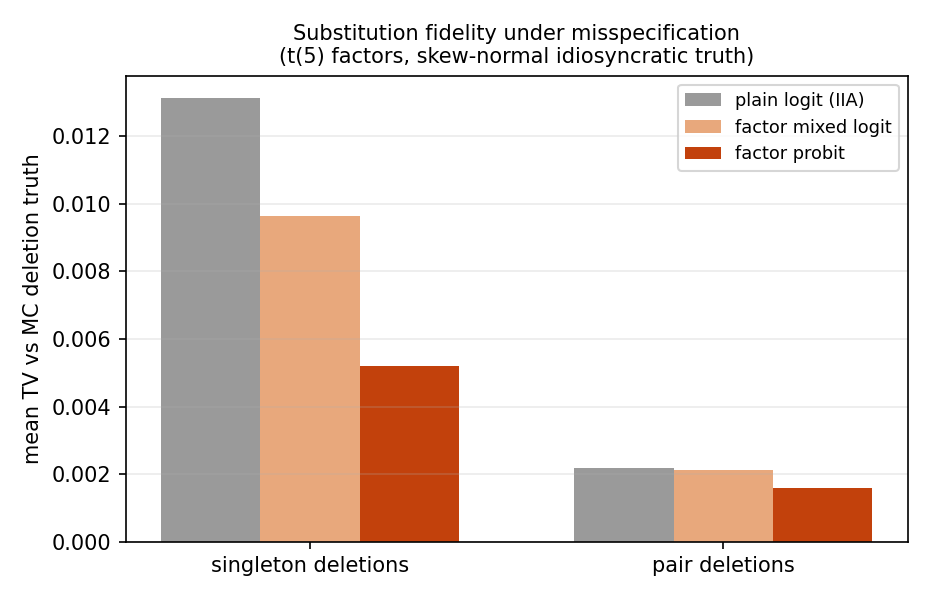
\includegraphics[width=0.48\textwidth]{figs/substitution.png}
\caption{Left: rank-$k$ approximation error under spectral decay $\gamma$
(dotted: GHK at $R=10^4$, per $\gamma$). Right: substitution fidelity with
standardized noise families, stratified by deleted share mass.}
\label{fig:boundary}
\end{figure}

\section{Related work}\label{sec:related}

GHK and simulated likelihood are standard
\cite{geweke1994,hajivassiliou1998,train2009}; analytic-approximation lines
include MACML \cite{bhat2011}; modern Gaussian-probability methods include
minimax tilting \cite{botev2017}. Factor dimension reduction for probit is
classical: Butler--Moffitt one-factor quadrature \cite{butler1982},
Elrod--Keane factor-analytic probit \cite{elrod1995}, and the probit
probability approximations surveyed in \cite{connors2014}. The lattice
survival-product identity and its inverse transform are from
\cite{cotton2021}. The novelty claimed here is the all-alternatives assembly
with inversion and removal-ensemble reuse --- not dimensional reduction, which
is old. Share inversion and its acceleration are central to demand estimation
\cite{berry1995,conlon2020}; automatic differentiation of logit-based BLP is
recent \cite{chia2021}; a 2026 preprint approximates correlated-choice
probabilities with equivariant neural networks \cite{huch2026}, evidence of
current demand for this computation. We are unaware of an automatically
differentiable, large-choice-set factor-probit demand implementation built on
deterministic share inversion; that precise object is what
Section~\ref{sec:discussion} proposes.

\section{Discussion}\label{sec:discussion}

Estimation is the natural next step: with the reduced coordinates of
Proposition~\ref{prop:ident}, gradients of an outer likelihood or GMM
objective pass through the share-inversion fixed point by implicit
differentiation, a candidate route to differentiable probit demand estimation
at large $N$. Estimating $(V, D)$ rather than supplying them raises the usual
identification cautions: utility scale normalization, factor rotation,
choice-invariant common loading components, and the fact that only difference
covariances are identified. Beyond the Gaussian family, the same machinery
computes races with arbitrary alternative-specific idiosyncratic densities; a
\emph{common-scale} Gumbel base with zero loadings reproduces the Luce model
exactly (alternative-specific scales break Luce, as they should), yielding
correlated-softmax generalizations. Finally, the inversion inherits the
original transform's interpolation structure (per-node location-to-probability
curves are cross-correlations, evaluable at all offsets simultaneously),
which we have not yet exploited.

\begin{thebibliography}{9}
\bibitem{geweke1994} J.~Geweke, M.~Keane, D.~Runkle. Alternative computational
approaches to inference in the multinomial probit model. \emph{Review of
Economics and Statistics} 76 (1994) 609--632.
\bibitem{hajivassiliou1998} V.~Hajivassiliou, D.~McFadden. The method of
simulated scores for the estimation of LDV models. \emph{Econometrica} 66
(1998) 863--896.
\bibitem{train2009} K.~Train. \emph{Discrete Choice Methods with Simulation},
2nd ed. Cambridge, 2009.
\bibitem{butler1982} J.~S. Butler, R.~Moffitt. A computationally efficient
quadrature procedure for the one-factor multinomial probit model.
\emph{Econometrica} 50 (1982) 761--764.
\bibitem{elrod1995} T.~Elrod, M.~P. Keane. A factor-analytic probit model for
representing the market structure in panel data. \emph{Journal of Marketing
Research} 32 (1995) 1--16.
\bibitem{bhat2011} C.~Bhat. The maximum approximate composite marginal
likelihood (MACML) estimation of multinomial probit-based unordered response
choice models. \emph{Transportation Research B} 45 (2011) 923--939.
\bibitem{connors2014} R.~Connors, S.~Hess, A.~Daly. Analytic approximations
for computing probit choice probabilities. \emph{Transportmetrica A} 10
(2014) 119--139.
\bibitem{botev2017} Z.~Botev. The normal law under linear restrictions:
simulation and estimation via minimax tilting. \emph{JRSS-B} 79 (2017)
125--148.
\bibitem{cotton2021} P.~Cotton. Inferring relative ability from winning
probability in multientrant contests. \emph{SIAM J.\ Financial Mathematics}
12 (2021) 295--317.
\bibitem{berry1995} S.~Berry, J.~Levinsohn, A.~Pakes. Automobile prices in
market equilibrium. \emph{Econometrica} 63 (1995) 841--890.
\bibitem{conlon2020} C.~Conlon, J.~Gortmaker. Best practices for
differentiated products demand estimation with pyblp. \emph{RAND Journal of
Economics} 51 (2020) 1108--1161.
\bibitem{chia2021} A.~Chia. Automatically differentiable random coefficient
logistic demand estimation. arXiv:2106.04636 (2021).
\bibitem{huch2026} E.~Huch, M.~Keane. Amortized inference for correlated
discrete choice models via equivariant neural networks. arXiv:2603.24705
(2026).
\bibitem{allocationpkg} The \texttt{allocation} package: Thurstone-tilt
portfolio construction. \url{https://github.com/microprediction/allocation}.
\end{thebibliography}

\end{document}
